%%%%%%%%%%%%%%%%%%%%%%%%%%%%%%%%%%%%%%%%%
% Arsclassica Article
% LaTeX Template
% Version 1.1 (10/6/14)
%
% This template has been downloaded from:
% http://www.LaTeXTemplates.com
%
% Original author:
% Lorenzo Pantieri (http://www.lorenzopantieri.net) with extensive modifications by:
% Vel (vel@latextemplates.com)
%
% License:
% CC BY-NC-SA 3.0 (http://creativecommons.org/licenses/by-nc-sa/3.0/)
%
%%%%%%%%%%%%%%%%%%%%%%%%%%%%%%%%%%%%%%%%%

%----------------------------------------------------------------------------------------
%	PACKAGES AND OTHER DOCUMENT CONFIGURATIONS
%----------------------------------------------------------------------------------------

\documentclass[
10pt, % Main document font size
a4paper, % Paper type, use 'letterpaper' for US Letter paper
oneside, % One page layout (no page indentation)
%twoside, % Two page layout (page indentation for binding and different headers)
headinclude,footinclude, % Extra spacing for the header and footer
BCOR5mm, % Binding correction
]{scrartcl}

%----------------------------------------------------------------------------------------

\usepackage{listings} % Required for inserting code snippets
\usepackage[usenames,dvipsnames]{xcolor} % Required for specifying custom colors and referring to colors by name
\usepackage[titletoc,title]{appendix}
\usepackage{ amssymb }
\usepackage{hyperref}

\definecolor{DarkGreen}{rgb}{0.0,0.4,0.0} % Comment color
\definecolor{highlight}{RGB}{255,251,204} % Code highlight color

\lstdefinestyle{Style1}{ % Define a style for your code snippet, multiple definitions can be made if, for example, you wish to insert multiple code snippets using different programming languages into one document
language=Fortran, % Detects keywords, comments, strings, functions, etc for the language specified
backgroundcolor=\color{highlight}, % Set the background color for the snippet - useful for highlighting
basicstyle=\footnotesize\ttfamily, % The default font size and style of the code
breakatwhitespace=false, % If true, only allows line breaks at white space
breaklines=true, % Automatic line breaking (prevents code from protruding outside the box)
captionpos=b, % Sets the caption position: b for bottom; t for top
commentstyle=\usefont{T1}{pcr}{m}{sl}\color{DarkGreen}, % Style of comments within the code - dark green courier font
deletekeywords={}, % If you want to delete any keywords from the current language separate them by commas
%escapeinside={\%}, % This allows you to escape to LaTeX using the character in the bracket
firstnumber=1, % Line numbers begin at line 1
frame=single, % Frame around the code box, value can be: none, leftline, topline, bottomline, lines, single, shadowbox
frameround=tttt, % Rounds the corners of the frame for the top left, top right, bottom left and bottom right positions
keywordstyle=\color{Blue}\bf, % Functions are bold and blue
morekeywords={}, % Add any functions no included by default here separated by commas
numbers=left, % Location of line numbers, can take the values of: none, left, right
numbersep=10pt, % Distance of line numbers from the code box
numberstyle=\tiny\color{Gray}, % Style used for line numbers
rulecolor=\color{black}, % Frame border color
showstringspaces=false, % Don't put marks in string spaces
showtabs=false, % Display tabs in the code as lines
stepnumber=5, % The step distance between line numbers, i.e. how often will lines be numbered
stringstyle=\color{Purple}, % Strings are purple
tabsize=2, % Number of spaces per tab in the code
}

%%%%%%%%%%%%%%%%%%%%%%%%%%%%%%%%%%%%%%%%%
% Arsclassica Article
% Structure Specification File
%
% This file has been downloaded from:
% http://www.LaTeXTemplates.com
%
% Original author:
% Lorenzo Pantieri (http://www.lorenzopantieri.net) with extensive modifications by:
% Vel (vel@latextemplates.com)
%
% License:
% CC BY-NC-SA 3.0 (http://creativecommons.org/licenses/by-nc-sa/3.0/)
%
%%%%%%%%%%%%%%%%%%%%%%%%%%%%%%%%%%%%%%%%%

%----------------------------------------------------------------------------------------
%	REQUIRED PACKAGES
%----------------------------------------------------------------------------------------

\usepackage[
nochapters, % Turn off chapters since this is an article        
beramono, % Use the Bera Mono font for monospaced text (\texttt)
eulermath,% Use the Euler font for mathematics
pdfspacing, % Makes use of pdftex’ letter spacing capabilities via the microtype package
dottedtoc % Dotted lines leading to the page numbers in the table of contents
]{classicthesis} % The layout is based on the Classic Thesis style

\usepackage{arsclassica} % Modifies the Classic Thesis package

\usepackage[T1]{fontenc} % Use 8-bit encoding that has 256 glyphs

\usepackage[utf8]{inputenc} % Required for including letters with accents

\usepackage{graphicx} % Required for including images
\graphicspath{{Figures/}} % Set the default folder for images

\usepackage{enumitem} % Required for manipulating the whitespace between and within lists

\usepackage{lipsum} % Used for inserting dummy 'Lorem ipsum' text into the template

\usepackage{subfig} % Required for creating figures with multiple parts (subfigures)

\usepackage{amsmath,amssymb,amsthm} % For including math equations, theorems, symbols, etc

\usepackage{varioref} % More descriptive referencing

%----------------------------------------------------------------------------------------
%	THEOREM STYLES
%---------------------------------------------------------------------------------------

\theoremstyle{definition} % Define theorem styles here based on the definition style (used for definitions and examples)
\newtheorem{definition}{Definition}

\theoremstyle{plain} % Define theorem styles here based on the plain style (used for theorems, lemmas, propositions)
\newtheorem{theorem}{Theorem}

\theoremstyle{remark} % Define theorem styles here based on the remark style (used for remarks and notes)

%----------------------------------------------------------------------------------------
%	HYPERLINKS
%---------------------------------------------------------------------------------------

\hypersetup{
%draft, % Uncomment to remove all links (useful for printing in black and white)
colorlinks=true, breaklinks=true, bookmarks=true,bookmarksnumbered,
urlcolor=webbrown, linkcolor=RoyalBlue, citecolor=webgreen, % Link colors
pdftitle={}, % PDF title
pdfauthor={\textcopyright}, % PDF Author
pdfsubject={}, % PDF Subject
pdfkeywords={}, % PDF Keywords
pdfcreator={pdfLaTeX}, % PDF Creator
pdfproducer={LaTeX with hyperref and ClassicThesis} % PDF producer
}
 % Include the structure.tex file which specified the document structure and layout

\hyphenation{Fortran hy-phen-ation} % Specify custom hyphenation points in words with dashes where you would like hyphenation to occur, or alternatively, don't put any dashes in a word to stop hyphenation altogether

\setcounter{secnumdepth}{5}


% Create a command to cleanly insert a snippet with the style above anywhere in the document
\newcommand{\insertcode}[2]{\begin{itemize}\item[]\lstinputlisting[caption=#2,label=#1,style=Style1]{#1}\end{itemize}} % The first argument is the script location/filename and the second is a caption for the listing

%----------------------------------------------------------------------------------------
%	TITLE AND AUTHOR(S)
%----------------------------------------------------------------------------------------

\title{\normalfont\spacedallcaps{Molecular dynamics simulation of Argon}} % The article title

\author{\spacedlowsmallcaps{Alexander Cronheim\textsuperscript{1} \& Aboubakr El Mahdaoui\textsuperscript{1}}} % The article author(s) - author affiliations need to be specified in the AUTHOR AFFILIATIONS block

\date{} % An optional date to appear under the author(s)

%----------------------------------------------------------------------------------------

\begin{document}

%----------------------------------------------------------------------------------------
%	HEADERS
%----------------------------------------------------------------------------------------

\renewcommand{\sectionmark}[1]{\markright{\spacedlowsmallcaps{#1}}} % The header for all pages (oneside) or for even pages (twoside)
%\renewcommand{\subsectionmark}[1]{\markright{\thesubsection~#1}} % Uncomment when using the twoside option - this modifies the header on odd pages
\lehead{\mbox{\llap{\small\thepage\kern1em\color{halfgray} \vline}\color{halfgray}\hspace{0.5em}\rightmark\hfil}} % The header style

\pagestyle{scrheadings} % Enable the headers specified in this block

%----------------------------------------------------------------------------------------
%	TABLE OF CONTENTS & LISTS OF FIGURES AND TABLES
%----------------------------------------------------------------------------------------

\maketitle % Print the title/author/date block

\setcounter{tocdepth}{3} % Set the depth of the table of contents to show sections and subsections only

%\tableofcontents % Print the table of contents

%\listoffigures % Print the list of figures

%\listoftables % Print the list of tables

{\let\thefootnote\relax\footnotetext{\textsuperscript{1} \textit{Faculty of Applied Physics, University of Techonology, Delft, the Netherlands}}}

%\newpage % Start the article content on the second page, remove this if you have a longer abstract that goes onto the second page

%----------------------------------------------------------------------------------------
%	ABSTRACT
%----------------------------------------------------------------------------------------

\newpage

\section*{Abstract} % This section will not appear in the table of contents due to the star (\section*)

The motion of a collection of 864 particles has been simulated in Fortran using Molecular Dynamics techniques to compute values for pressure, specific heat and the static pair correlation function with density and temperature as input paramters. The computed properties were compared with experimental results for the properties of argon. The simulation was done with a Lennard-Jones pair-potential and the system was allowed to reach equilibrium. The computed results are in relative good agreement with the known properties of argon.

%\lipsum[1] % Dummy text

%----------------------------------------------------------------------------------------
%	AUTHOR AFFILIATIONS
%----------------------------------------------------------------------------------------

%{\let\thefootnote\relax\footnotetext{* \textit{Faculty of Applied Physics, University of Techonology, Delft, the Netherlands}}}


%----------------------------------------------------------------------------------------

%\newpage % Start the article content on the second page, remove this if you have a longer abstract that goes onto the second page

%----------------------------------------------------------------------------------------
%	INTRODUCTION
%----------------------------------------------------------------------------------------
\newpage

\section{Introduction}

%In this report we discuss the results of simulations for a system of argon gas with 864 particles. 

Molecular dynamics is a method to simulate a many-particle system by numerically solving Newton's classical equations of motion for all particles for a period of time. The main limitations are the fact that simulations are only  realizable for small systems  and times compared to experimental systems in general. %Furthermore, the systems to be simulated can only be classical in the usual molecular dynamics approach. 
The simulations consist of monatomic particles subjected to pair interaction forces that result from a Lennard-Jones \ref{eq:lennard-jones} potential.  
%A Lennard-Jones Potential is implemented for the calculation of the force between the particles where a pair potential is assumed. 
This is reported to be in good agreement with experimental results in the case of argon \cite{Verlet:1967md}.
 

After initialization
%with the particles in a FCC latice structure and velocities according to the Maxwell Boltzman distribution,
the system's equations of motion are solved numerically for each time step using the velocity Verlet algorithm.  Because the systems initial state differs from the equilibrium state, the system is first allowed to relax to equilibrium. Because the simulation is run in the microcanonical ensemble, i.e. at constant energy and volume with a fixed number of particles, the system must be moved towards the intended temperature. For that a simple thermostat algorithm that rescales the velocities is used until the system has settled at the intended temperature. 

When the desired equilibrium state has been reached, the simulation continues and collects results for calculating the time average of different properties of the system. The equipartition theorem is used for calculating the temperature, the virial theorem is applied in the calculation of the pressure, specific heat is evaluated using a formula derived by Lebowitz using the fluctuations of the kinetic energy\cite{Duane:1985lz}.



 
\newpage


%----------------------------------------------------------------------------------------
%	METHODS
%----------------------------------------------------------------------------------------

\section{Methods for Simulation}
The Lennard Jones pair potential is used to describe the interaction between a pair of atoms and models a repulsive term and an attractive term as a function of separation distance $r_{ij}$.

\begin{equation}
V_{ij} =  4 \epsilon \left [ \left (\frac{\sigma}{r_{ij}} \right )^{12} - \left ( \frac{\sigma}{r_{ij}} \right )^6 \right ]
\label{eq:lennard-jones}
\end{equation}

Here $\epsilon$ and $\sigma$ determine respectively the depth of the potential well and the characteristic separation distance between two particles where the potential is zero. A particle pairs relative position is denoted by $\mathbf{r_{ij}}$. For argon this has been working quite well as a good mathematical model for all three phases\cite{Rahman}.

%\subsection{Reduced units}
In order to decrease numerical errors $\epsilon$ and $\sigma$ reduced units are used throughout the simulation, with energy described in units of $\epsilon$,  distance in $\sigma$, and mass in units of particle mass $m$.  Then the reduced unit of time is: $\sigma(m/\epsilon)^{1/2}$.
By setting the Boltzman constant $k_B$ equal to one in the simulation, the temperature is transferred to a description in units of $\epsilon / k_B$.

\subsection{Initialization}

The particles are initialized in a cubic geometry according to an FCC-lattice structure, consistent with the fact that the ground state configuration is an FCC lattice for argon. Considering that a cubic FCC-cell contains four particles, and setting the number of cells per cartesian dimension to six results in 864 particles.

%The particles initial velocities are drawn from a Maxwell Boltzman distribution. 
% , 


%The system is initialized by creating an fcc lattice structure and assigning each position of the particles to the lattice points. This is done for 864 particles but can in principle be easily implemented for a number of particles $N$ that can be written as $4M^3$ with $M$ an integer and representing the number of fcc cells in one dimension.

%\insertcode{"Scripts/initialization_snippet_1.f90"}{Constructing the fcc lattice} % The first argument is the script location/filename and the second is a caption for the listing

%Above can you see the code with $i$, $j$ and $k$ for the $x$, $y$ and $z$ component and a function fcc\_cell is called that takes an argument $l$ to add the relative position of each particle in a particular cell.


%\subsubsection{Velocity Distribution}

The particles are then assigned an initial velocity that is randomly distributed according to the Maxwell-Boltzmann distribution. A property of this distribution is that each (cartesian) velocity component obeys a Gaussian distribution with zero mean \ref{eq:boltzgauss}:

\begin{equation} f(v_i) = \sqrt{\frac{m}{2\pi k_B T}} e^{\frac{-mv_i^2}{2k_BT}} 
\label{eq:boltzgauss}
\end{equation}

%\insertcode{"Scripts/initialization_snippet_2.f90"}{Generating initial velocities} % The first argument is the script location/filename and the second is a caption for the listing

%\insertcode{"Scripts/initialization_snippet_3.f90"}{Removing the center of mass degree of freedom} % The first argument is the script location/filename and the second is a caption for the listing

Uniformly distributed random numbers are drawn from the intrinsic Fortran random-number subroutine. The seed for the random number generator is provided by a script from the ICCP coding manual\cite{Glosser:2015iccp} based on the entropy collected by the computer. The Box muller transform is applied to convert two random variables drawn from a uniform distribution to a random variable that is normally distributed.

After assignment of the random initial velocities the center of mass velocity is set to zero by substracting from each particle the system's total average velocity. This is in order to avoid introducing an offset in the kinetic energy calculation.

\subsection{Boundary Conditions}
As the system to be simulated is very small compared to real experimental systems, boundaries would probably have a profound effect in the simulation. 
To counter this periodic boundary conditions are used. This is implemented by copying the system in all directions creating a large box of 9 identical smaller boxes with the middle box our system of interest. Whenever a particle leaves the original system, it must reappear on the exact opposite side with the same velocity vector.

As we calculate the forces the Lennard Jones pair potential is evaluated for all the particles inside the box and also all the other 8 copies that are closer than a predefined cut off distance. 
The latter is needed as long range interactions would otherwise result in a non periodic potential. This can be done because the potential tends to zero for large $r_{ij}$.


%\insertcode{"Scripts/boundary_conditions_snippet_1.f90"}{Creating periodic boundary conditions} % The first argument is the script location/filename and the second is a caption for the listing


\subsection{Interaction forces}
Only pair wise interaction forces are considered between each particle pair: $\mathbf{F_{ij}} = - \nabla V_{ij}$. The force on each particle is then calculated as \ref{eq:particleforce}:
\begin{equation}
\mathbf{F_{i}} = \sum_{j \neq i} \epsilon \left ( 48 \frac{\sigma^{12}}{r_{ij}^{14}} - 24 \frac{\sigma^6}{r_{ij}^8} \right ) \mathbf{r_{ij}} 
\label{eq:particleforce}
\end{equation}
The sum runs over all particle pairs within the cut off distance of the potential in the original system and its neighboring copies.
Setting the potential cut off distance to half the length of the original system results in evaluating only the nearest instance of a particle and its copies.

\subsection{Time integration}
The systems evolution of time is calculated by numerically integrating Newton's equations of motion over discrete timesteps $h$. The particles velocity and postion at each time step is calculated with the velocity Verlet algorithm: 

\begin{align}
\tilde{\mathbf{v}}(t) &=  \mathbf{v}(t) + h \mathbf{F}(t)/2 \\
\mathbf{r}(t+h) &= \mathbf{r}(t) + h\tilde{\mathbf{v}}(t) \\
\mathbf{v}(t+h) &= \tilde{\mathbf{v}}(t) + h \mathbf{F}(t+h)/2 
\end{align}

This algorithm belongs to the class of symplectic integration methods, which if implemented correctly conserve energy. The accumulated error in position and velocity is of order $h^2$, this is an order more accurate than the simpler semi-implicit Euler method.

\subsection{Temperature}

The systems temperature $T$ is related to the kinetic energy $K$ through the equipartition theorem \ref{eq:equipartition} for a monoatomic ideal gas. 
 \begin{equation} 
 \label{eq:equipartition}
 K = \frac{3}{2} (N - 1) k_B T
 \end{equation}
The number of degrees of freedom is $3/2$ times the number of particles $N$. The center of mass degrees of freedom are substracted as these are fixed in a microcanonical system with periodic boundary conditions and no external interactions, following an argument in \cite{Thijssen:2013cp}

%, the center of mass degree of freedom is not available in a micro canonical molecular dynamics simulation, hence the $N-1$ in equation \ref{eq:equipartition}. This is used to calculate the temperature of the system.

%The equipartition theorem is applicable that every systems  states that each per degree of freedom the contribution to the kinetic energy $E_{kin}$ is proportional to $1/2 k_B T$.

In order to move the system towards the intended temperature, all the particles velocities are rescaled by multiplying them with a scaling factor $\lambda$, which is the square root of the ratio between the kinetic energy corresponding to the intended temperature $T$ and the systems current kinetic energy, following \cite{Thijssen:2013cp}:
\begin{equation} 
\lambda = \sqrt{ \frac{3 (N-1) k_BT}{ \sum_{i=1}^N mv_i^2} } 
\end{equation}



\subsection{Pressure}

Because there are no walls in a system with periodic boundary conditions, the virial theorem is used for measuring the pressure in the simulation. In a pair potential the virial theorem can be described according to equation \ref{eq:virial}, with $\frac{\delta U(R)}{\delta r_{ij}} = \mathbf{r_{ij}} \cdot \mathbf{f_{ij}}$. 

\begin{equation} 
\frac{\beta P}{\rho} = 1 + \frac{\beta}{3N} \left \langle \sum_i \sum_{j>i} \mathbf{r_{ij}} \cdot \mathbf{f_{ij}} \right \rangle 
\label{eq:virial}
\end{equation}

Here $\beta$ is shorthand for $1/k_B T$.The brackets denote an ensemble average, however, in our simulation, we take the time average instead. Actually, because the simulation is run in the microcanonical regime, the ensemble average, in our case the time average, must be used for the temperature, which for every timestep is calculated using the equipartition theorem \ref{eq:equipartition}.


\subsubsection{Specific Heat}

%The specific heat at constant volume $C_V$  is defined as:
%\begin{equation} C_V = \left ( \frac{\delta E}{\delta T} \right )_V %\end{equation}

%\noindent
%In molecular dynamics simulations, a quantity that can be calculated is the %ensemble average of the total energy $\langle E\rangle_{NVT}$:

%\begin{equation} \langle E\rangle_{NVT} = \frac{ \sum_X e^{-\beta \mathcal{H}(X)} %\mathcal{H}(X)}{ \sum_X e^{-\beta \mathcal{H}(X)}} = - \frac{\delta ln(Z)}{\delta %\beta} \end{equation}

%\noindent
%Using the ensemble average for the total energy, the formula for the specific %heat can be rewritten as a function of the fluctuations in the total energy:

%\begin{align}
%C_V &= \frac{1}{k_B T^2} \frac{\delta^2 ln(Z)}{\delta \beta^2} \\
%&= \frac{1}{k_B T^2} \left ( \langle E^2\rangle_{NVT} - \langle E\rangle^2_{NVT} %\right )
%\end{align}

%\noindent
%This is still difficult to use in a program simulating a system in the microcanonical ensemble as the total energy is kept fixed, but following the derivation by Lebowitz\cite{Duane:1985lz} this can be related to the fluctuation in kinetic energy:

In the canonical ensemble one can derive the specific heat by measuring the fluctuations of the total energy, as is well known in the field of statistical mechanics. 
However in the microcanonical ensemble of which our simulated system is an example, there should be no fluctiations as the total energy is kept fixed.
Following the derivation by Lebowitz\cite{Duane:1985lz} which relates the specific heat to fluctuations in kinetic energy, we can calculate the specific heat using the fluctuations in kinetic energy.

%\begin{equation}
%C_V = \frac{1}{k_B T^2} \left ( \langle E^2\rangle - \langle E\rangle^2 \right )
%\end{equation}


\begin{equation} 
\frac{\langle\delta K^2\rangle}{\langle K\rangle^2} = \frac{2}{3N} \left ( 1 - \frac{3N}{2C_V} \right ) 
\end{equation}

%The implementation in our simulation is inside the algorithm for the dynamics of the particles. For each time step the new velocities are calculated, the kinetic energy is also calculated and the relevant sums of the kinetic energy are updated in a subroutine "calc\_specific\_heat":

%\insertcode{"Scripts/specific_heat_snippet_1.f90"}{Updating the relevant sums of the kinetic energy} % The first argument is the script location/filename and the second is a caption for the listing

%\noindent
%As discussed earlier, the specific heat is related to the fluctuations in kinetic energy using a formula derived by Lebowitz\cite{Duane:1985lz}:

%\begin{equation} \frac{\langle\delta K^2\rangle}{\langle K\rangle^2} = \frac{2}{3N} \left ( 1 - \frac{3N}{2C_V} \right ) \end{equation}

%\noindent
%Rewriting this to get an expression for the specific heat:

%\begin{equation}
%C_V = \left (\frac{2}{3N} - \frac{\langle K^2 \rangle - \langle K \rangle^2}{\langle K\rangle^2} \right )^{-1} 
%\end{equation}

%where again the time average is taken instead of the ensemble average.

%\noindent
%Using the time average instead of the ensemble average, the averages can be expressed as a sum over all time steps $n_t$ divided by the time steps:
%\begin{equation} \langle K^2 \rangle  = \frac{\sum_{i=1}^{n_t} K(i)^2}{n_t} \end{equation}
%\begin{equation} \langle K \rangle^2  = \left ( \frac{\sum_{i=1}^{n_t} K(i)  }{n_t} \right)^2 %\end{equation}

%\noindent
%Now the specific heat can be calculated as:
%\begin{align}
%C_V &= \left (\frac{2}{3N} - \frac{\langle K^2 \rangle - \langle K \rangle^2}{\langle K\rangle^2} \right )^{-1} \\
%&= \left ( \frac{2}{3N} - \frac{\sum_{i=1}^{n_t} K(i)^2*n_t - \left (\sum_{i=1}^{n_t} K(i) \right )^2 }{\left (\sum_{i=1}^{n_t} K(i) \right )^2 } \right )^{-1}
%\end{align}

%This is implemented in our code within the same subroutine "calc\_specific\_heat" after an if statement is enabled at the end of the simulation:
%\insertcode{"Scripts/specific_heat_snippet_2.f90"}{Calculating the specific heat} % The first argument is the script location/filename and the second is a caption for the listing


\subsubsection{Pair Correlation Function}

The static pair correlation function in the canonical ensemble can be expressed as:

\begin{equation} g(\mathbf{r,r'}) = V^2 \frac{1}{N!h^{3N}Z} \int_V d^3r_3....d^3r_N e^{-\beta V_N(\mathbf{r,r',r_3.....r_N})} \end{equation}

noindent
If the system is homogeneous and has a large number of particles $N$, it can also be written as a function of the difference $\mathbf{\Delta r} = \mathbf{r} - \mathbf{r'}$:

\begin{equation} g(\mathbf{\Delta r}) = \frac{V}{N(N-1)}  \left \langle \int d^3r' \sum_{i,j i \neq j}^N \delta(\mathbf{r}-\mathbf{r}_i) \delta(\mathbf{r'} + \Delta\mathbf{r} - \mathbf{r}_j) \right \rangle \end{equation}

The pair correlation function \ref{eq:corr} can be evaluated in molecular dynamics systems  if a histogram is recorded of the number of pairs of particles $n(r)$ for each distance $r$: 

\begin{equation} 
g(r) = \frac{2V}{N(N-1)} \left [ \frac{\langle n(r) \rangle }{ 4 \pi r^2 \Delta r} \right ] 
\label{eq:corr}
\end{equation}

\noindent
Where $V = L^3$ denotes the volume of the system. In our simulation a number of intervals $n_i$ is defined which together with the length in each direction $L$ sets the small $\Delta r$:

\begin{equation} \Delta r  = \frac{L}{n_i} \end{equation}

%\noindent
%Again a time average is used and the average number of pairs $\langle n(r) \rangle $ is calculated as a sum of all the pair occurences $N(r,t)$ in a time step $t$ and in a distance $r$ over all time steps $n_t$:
%\begin{equation} \langle n(r) \rangle = \frac{\sum_t^{n_t} N(r,t)}{n_t} \end{equation}

\noindent
For a large enough number of intervals the distance $r$ can be approximated by $i\Delta r$ with $i$ the index of the corresponding interval. The number of pair occurrences $N(r,t)$ in a time step $t$ and in a distance $r$ can be expressed now as function of the interval you are in $N(i,t)$. This way we are able to count all pair occurrences in our program and calculate the pair correlation function:

\begin{align}
g(r) &\approx \frac{2V}{N(N-1)} \left [ \frac{\langle n(r) \rangle }{ 4 \pi r^2 \Delta r} \right ] \\
&= \frac{2L^3}{N(N-1)} \left [ \frac{\sum_t^{n_t} N(i,t)}{n_t 4 \pi i^2 \Delta r^2 \Delta r} \right ] \\
&= \frac{2L^3}{N(N-1)} \frac{\sum_t^{n_t} N(i,t)}{n_t 4 \pi i^2} \frac{n_i^3}{L^3} \\
&= \frac{2}{N(N-1)} \frac{n_i^3}{n_t 4 \pi} \frac{\sum_t^{n_t} N(i,t)}{i^2}
\end{align}

\noindent
This is implemented in the code as follows. For each interval $i$ the number of pair occurrences in that interval is registered in a particular time interval. This is done while evaluating the forces of the particles.
%\insertcode{"Scripts/pair_correlation_snippet_1.f90"}{Updating the histogram for each interval} % The first argument is the script location/filename and the second is a caption for the listing

%\noindent
%As the final time step is done and the routine for the dynamics is finished, the sum for each interval is passed to a routine for calculating the pair correlation function that is called at the end:
%\insertcode{"Scripts/pair_correlation_snippet_2.f90"}{Factors are needed to prevent overflow errors} % The first argument is the script location/filename and the second is a caption for the listing


\subsection{Data blocking}

When estimating the statistical measurement error, one would calculate the standard deviation of an ensemble of independent realisations of the same observable. In our case, every measurement is based on the time average of not uncorrelated realisations of instanteneous observables. Because of this one should also take the correlation time of these observables into account. 

A simpler method exists however, it amounts to dividing the correlated dataset into blocks of equal length larger than the correlation time. Then, the time averages of the measurements over a single block can be regarded as independent from the other blocks. Subsequently the error can be estimated as the standard deviation of the averages of the different blocks. 

%----------------------------------------------------------------------------------------
%	RESULTS AND DISCUSSION
%----------------------------------------------------------------------------------------
\newpage

\section{Results and Discussion}

%stepsize
%No time steps, velocity rescaling steps, equilibriation steps, data block size.
%summary results table. literature table, LJ potential constants for argon in introduction, references.
%binsize for histogram..


\subsection{Energy}
Since the simulation is run in the microcanonical regime, apart from some velocity rescaling in the equilibriation phase, the total energy should be conserved, while the potential and kinetic energy are allowed to fluctuate and this can be seen in Figure \ref{fig:energy-evolution}. Due to numerical errors, the total energy does fluctuate a bit, but to a much lesser degree than the kinetic and potential energy do. 

\begin{figure}[h]
\centering
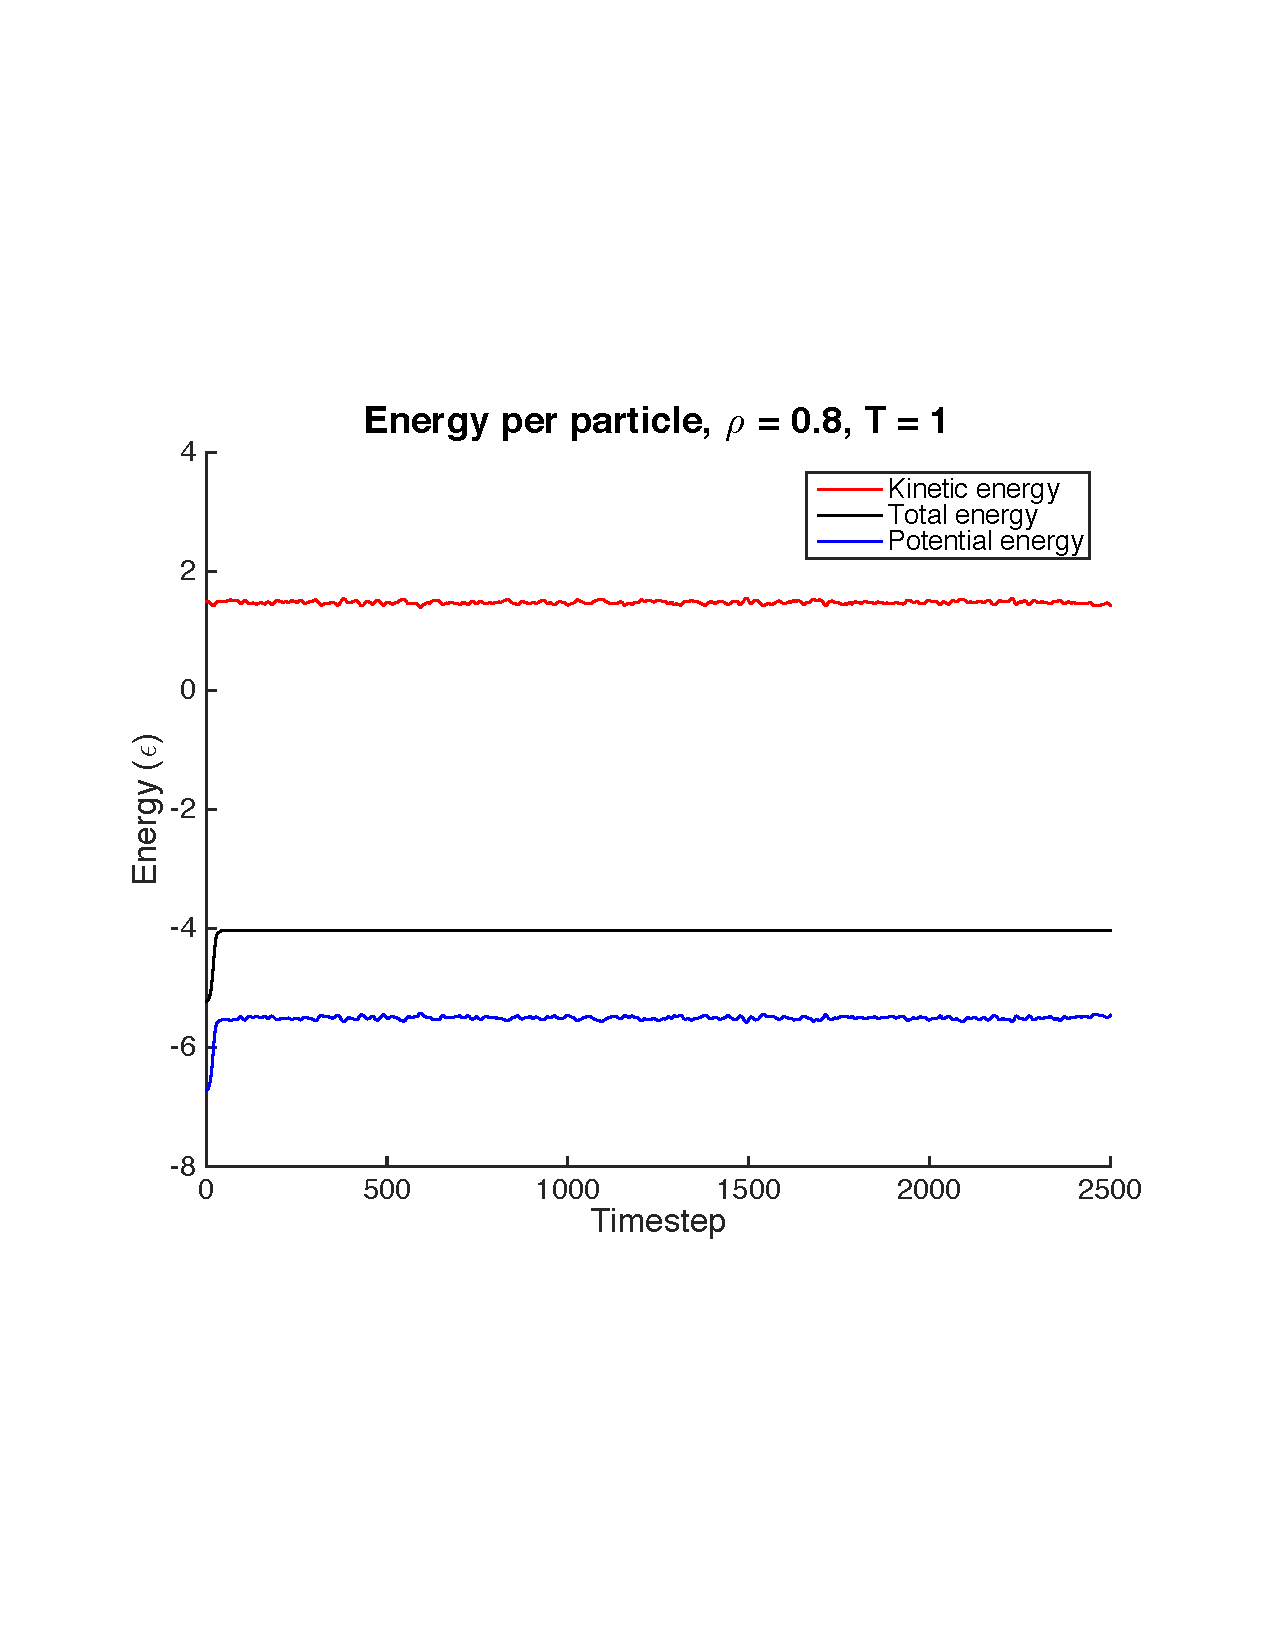
\includegraphics[width=0.6\textwidth]{energy-evolution-rho08-T10.pdf}
\caption{Time evolution of the energies of the system. Note the effect of velocity rescaling in the equilibration phase. Here the fluctuations of the potential and kinetic energy are in the order of $2.43\cdot10^{-02}$ $\epsilon$, while those of the total energy are in the order of $6.34\cdot10^{-05}$  $\epsilon$.}
\label{fig:energy-evolution}
\end{figure}

\newpage


\subsection{Macroscopic Thermodynamic Quantities}
In this section the results for pressure, temperature and the specific heat are presented in Table~\vref{tab:label} and is compared with the values of Verlet'spaper\cite{Verlet:1967md} and Table ~\vref{tab:label2} for molecular dynamics simulations of a Lennard Jones liquid in \cite{Thijssen:2013cp}


\begin{table}[hbt]
\caption{Thermodynamic quantities of the Lennard–Jones particles.}
\centering
\begin{tabular}{llllll}
\toprule
\toprule
%\multicolumn{2}{c}{Name} \\
%\cmidrule(r){1-2}
$\rho(1/\sigma^3)$ & $T_0(\epsilon/k_B)$ & $T$ & $\beta P/\rho$ & $U(\epsilon)$ & $C_V$\\
\midrule
$0.3 $ & $3.0$ & $3.233(7) $ & $ 1.16(2)$ & $-1.71(1)$ & $1.64(4)$\\
$0.7 $ & $0.3$ & $0.51(7)$ & $-3(2)$ & $-5.6(1)$ & $-0(5)$\\
$0.7 $ & $0.5$ & $0.58(3)$ & $-2.8(8)$ & $-5.29(5)$ & $-0.3(7)$\\
$0.7 $ & $0.7$ & $0.715(7)$ & $-1.8(1)$ & $-5.06(1)$ & $2.8(4)$\\
$0.7 $ & $0.9$ & $0.920(5)$ & $-0.33(5)$ & $-4.910(7)$ & $2.1(2)$\\
$0.7$ & $1.0$ & $1.014(4)$ & $0.17(3)$ & $-4.842(5)$   & $2(1)$\\
$0.7 $ & $1.1$ & $1.090(7)$ & $ 0.46(7)$ & $-4.79(1)$ & $2.2(2)$\\
$0.7 $ & $1.5$ & $1.500(5)$ & $ 1.54(5)$ & $-4.546(8)$ & $2.0(2)$\\
$0.8 $ & $0.4$ & $0.45(2)$ & $-5(2)$ & $-6.23(3)$ & $-0(1)$\\
$0.8 $ & $0.6$ & $0.588(5)$ & $-2.3(1)$ & $-5.885(7)$ & $2.6(4)$\\
$0.8 $ & $0.8$ & $0.787(6)$ & $ 0.05(7)$ & $-5.678(9)$ & $2.4(4)$\\
$0.8$ & $1.0$ & $0.984(3)$ & $1.26(4)$ & $-5.503(5)$ & $2.3(4)$ \\
$0.8 $ & $1.1$ & $1.064(7)$ & $ 1.66(8)$ & $-5.43(1)$ & $2.5(5)$\\
$0.8 $ & $2.0$ & $2.018(5)$ & $ 3.35(3)$ & $-4.696(8)$ & $2.2(3)$\\
$0.88$ & $0.2$ & $0.256(0)$ & $-20.0(1)$ & $-7.151(1)$ & $2(1)$\\
$0.88$ & $0.3$ & $0.375(1)$ & $-10.9(3)$ & $-7.005(2)$ & $2.6(5)$\\
$0.88$ & $0.4$ & $0.498(3)$ & $-6.11(3)$ & $-6.855(5)$ & $3(1)$\\
$0.88$ & $0.5$ & $0.592(3)$ & $-3.77(3)$ & $-6.739(4)$ & $3(1)$\\
$0.88$ & $0.6$ & $0.680(5)$ & $-2.00(3)$ & $-6.611(8)$ & $2.7(8)$\\
$0.88$ & $0.7$ & $0.76(1)$ & $ 0.2(2)$ & $-6.37(2)$ & $6(2)$\\
$0.88$ & $0.8$ & $0.79(2)$ & $ 1.6(3)$ & $-6.20(3)$ & $-14.3(6)$\\ 
$0.88$ & $0.9$ & $0.847(8)$ & $ 2.33(9)$ & $-6.09(1)$ & $3.0(7)$\\
$0.88$ & $1.0$ & $0.977(6)$ & $2.90(7)$ & $-5.936(9)$ & $3(3)$ \\
$0.88$ & $1.1$ & $1.095(7)$ & $ 3.55(8)$ & $-5.80(1)$ & $2.4(7)$\\
$1.20$ & $0.5$ & $0.515(0)$ & $ 25.45(3)$ & $-7.373(0)$ & $2(4)$\\
\bottomrule
\bottomrule
\end{tabular}
\label{tab:label}
\end{table}

The results show relative good agreement with the reference data. The internal energies are very much comparable, the temperature shows that the thermostat is working quite well. As for the pressure, most data are in good agreement but some values diverge, for example at $\rho = 0.7$ and $T=1.0$ there is a drop in pressure that isn't reported in Table ~\vref{tab:label2}, but as will be discussed in the next section, it is clear that a phase transition is taking place going from $\rho =0.8$ to $\rho=0.6$ at $T=1.0$ from liquid argon to solid argon. This would explain the pressure drop and Verlet\cite{Verlet:1967md} shows a similar drop at $\rho = 0.65$. The transition from solid to liquid occurs at a lower than expected temperature in our simulation. This suggests a higher preference for the liquid state in our simulations. 



\begin{table}[hbt]
\caption{Reference data of thermodynamic quantities}
\centering
\begin{tabular}{lllll}
\toprule
\toprule
%\multicolumn{2}{c}{Name} \\
%\cmidrule(r){1-2}
$\rho(1/\sigma^3)$ & $T_0(\epsilon/k_B)$ & $T$ & $\beta P/\rho$ & $U(\epsilon)$ \\
\midrule
$0.88$ & $1.0$ & $0.990$ & $ 2.98$ & $-5.704$ \\
$0.8 $ & $1.0$ & $1.010$ & $ 1.31$ & $-5.271$ \\
$0.7 $ & $1.0$ & $1.014$ & $ 1.06$ & $-4.662$ \\
\bottomrule
\bottomrule
\end{tabular}
\label{tab:label2}
\end{table}

The specific heat shows unexpected values and is relatively constant for higher temperatures en densities. This has probably to do with the fact that Lebowitz's formula uses the fluctuations in kinetic energy to evaluate the specific heat, but in our simulations the kinetic energy is fairly constant after relaxing to its equilibrium.




$$ C_V = \left (\frac{2}{3N} - \frac{\langle K^2 \rangle - \langle K \rangle^2}{\langle K\rangle^2} \right )^{-1} $$

%met 
%$$ \langle K^2 \rangle = \frac{\sum_i K(i)^2}{N_t} $$
%en 
%$$ \langle K \rangle^2 = \left (\frac{\sum_i K(i)}{N_t} \right )^2 $$

%En $N_t$ is het aantal tijdsstappen 

%------------------------------------------------


\subsection{Pair Correlation function}

The pair correlation function is plotted for $\rho = 0.88$ and different values of $T$ in Figure~\vref{fig:correlation}. It can be seen that the correlation function tends to 1 as expected in all cases. Furthermore, the repulsive term of the Lennard Jones potential prevents particles being close together as can be seen in the pair correlation. For $\rho = 0.88$, there is also a phase transition taking place between the temperatures $T=0.8$ and $T=0.6$ where solid argon shows a different pair correlation function with respect to liquid argon. 

For liquid argon the pair correlation function is simply oscillating indicating what the average distance is between  particles. As you move further away from a particular particle, the fluctuations in the average distances cause the peaks to broaden as well as the peaks to be lower for longer distances in the liquid argon. The solid argon shows peaks where the first, second etc. neighbors are in a lattice structure and shows a more complex function, but the oscillations tend to be more persistent even along longer distances compared to liquid argon as can be expected because of the periodic lattice structure. The results presented show good agreement with other experiments\cite{Thijssen:2013cp}. 

%The pair correlation function is plotted for $\rho = 0.88$ and $T=0.6$~\vref{fig:gallery}. It can be seen that this tends to 1 and is typical for solid argon. % The \vref command specifies the location of the reference

\begin{figure}[tb]
\centering
\subfloat[Pair correlation function of Argon($\rho = 0.88$, $T=0.4$) ]{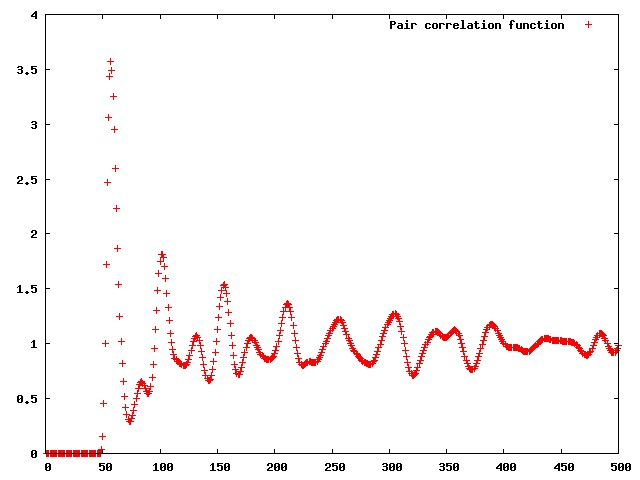
\includegraphics[width=.45\columnwidth]{histogramrho088T04}} \quad
\subfloat[Pair correlation function of Argon($\rho = 0.88$, $T=0.6$) ]{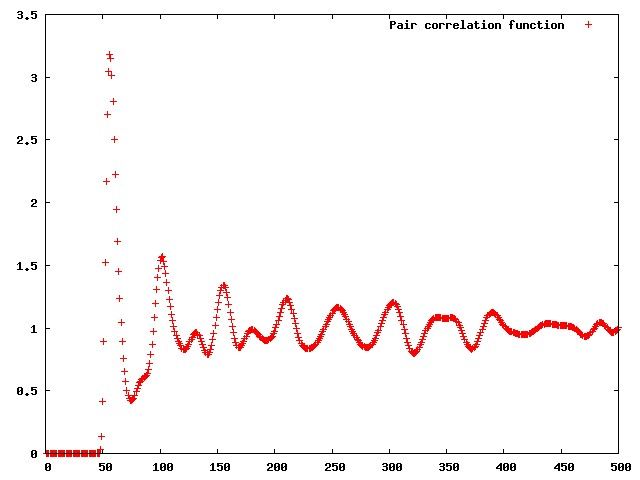
\includegraphics[width=.45\columnwidth]{histogramrho088T06}\label{fig:ipsum}} \\
\subfloat[Pair correlation function of Argon($\rho = 0.88$, $T=0.8$) ]{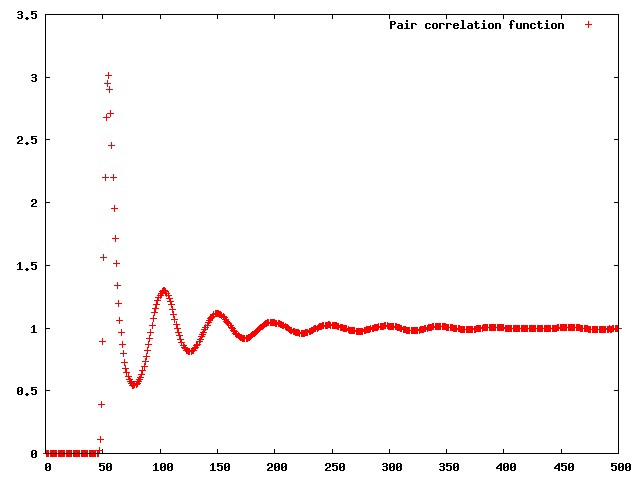
\includegraphics[width=.45\columnwidth]{histogramrho088T08}} \quad
\subfloat[Pair correlation function of Argon($\rho = 0.88$, $T=1.0$) ]{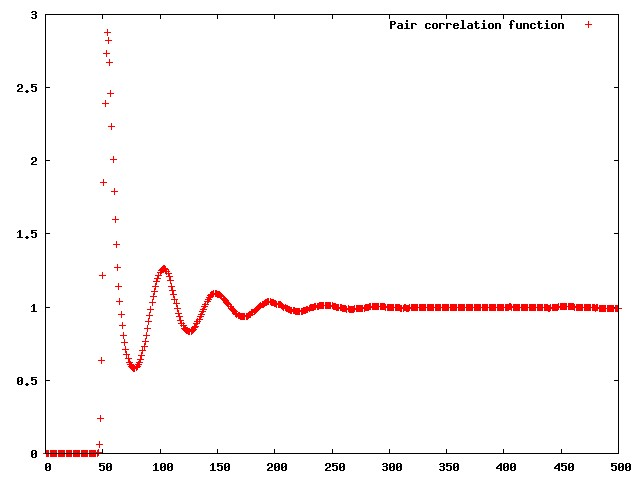
\includegraphics[width=.45\columnwidth]{histogramrho088T10}}
%\subfloat[Pair correlation function of Argon($\rho = 0.30$, $T=3.0$) ]{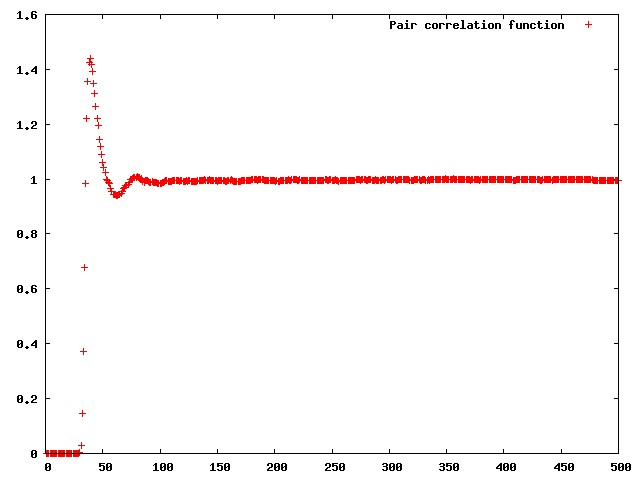
\includegraphics[width=0.5\columnwidth]{histogramrho030T30}}
\caption[Pair correlation function of Argon($\rho = 0.88$, $T=0.4-1.0$) ]{Phase transition shown in pair correlation} % The text in the square bracket is the caption for the list of figures while the text in the curly brackets is the figure caption
\label{fig:correlation}
\end{figure}


The simulation is also done for a higher temperature and lower density to observe the correlation function of argon in the gas phase. Results are shown in Figure~\vref{fig:gas-correlation} and show much less oscillations compared to liquid argon because of the increased disorder. This means that after the first peak where on average the first neighboring particle is present, the system is too disordered to show subsequent peaks.


\begin{figure}[tb]
\centering 
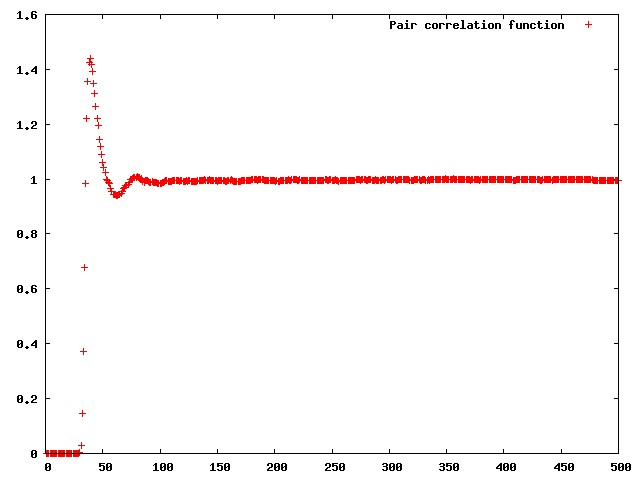
\includegraphics[width=0.5\columnwidth]{histogramrho030T30} 
\caption[Pair correlation function of Argon($\rho = 0.30$, $T=3.0$) ]{Pair correlation function of solid Argon ($\rho = 0.30$, $T=3.0$)} % The text in the square bracket is the caption for the list of figures while the text in the curly brackets is the figure caption
\label{fig:gas-correlation} 
\end{figure}

\subsection{Error estimation}
The estimated errors have been added in Table ~\vref{tab:label}. We have chosen a data block size of 200 time steps, because we observed the relaxation time to its equilibrium to be around a time scale less than 200 steps. We have to note that the relatively short simulation time of 2500 time steps compared to the blocks chosen has resulted in significant errors in our results. For future simulations we would recommend a longer simulation time to reduce the errors.





%------------------------------------------------


%----------------------------------------------------------------------------------------
%	BIBLIOGRAPHY
%----------------------------------------------------------------------------------------

\newpage
\newpage

\renewcommand{\refname}{\spacedlowsmallcaps{References}} % For modifying the bibliography heading

\bibliographystyle{unsrt}

\bibliography{sample.bib} % The file containing the bibliography

%----------------------------------------------------------------------------------------


%----------------------------------------------------------------------------------------
%	APPENDIX
%----------------------------------------------------------------------------------------

\newpage

\begin{appendices}

\section{Main Fortran source code}

%----------------------------------------------------------------------------------------

\insertcode{"../argon_box.f90"}{argon\_box.f90} % The first argument is the script location/filename and the second is a caption for the listing

%----------------------------------------------------------------------------------------

\newpage


\section{Fortran source code for setting the initial conditions}

%----------------------------------------------------------------------------------------

\insertcode{"../argon_box_init.f90"}{argon\_box\_init.f90} % The first argument is the script location/filename and the second is a caption for the listing

%----------------------------------------------------------------------------------------

\newpage


\section{Fortran source code for the dynamics of the system}

%----------------------------------------------------------------------------------------

\insertcode{"../argon_box_dynamics.f90"}{argon\_box\_dynamics.f90} % The first argument is the script location/filename and the second is a caption for the listing

%----------------------------------------------------------------------------------------

\newpage


\section{Fortran source code for output of results}

%----------------------------------------------------------------------------------------

\insertcode{"../argon_box_results.f90"}{argon\_box\_results.f90} % The first argument is the script location/filename and the second is a caption for the listing

%----------------------------------------------------------------------------------------

\newpage

\end{appendices}

\end{document}






